\utsection{OpenBTS Software-Architektur}{Stefan Giggenbach}\label{sec:swarch}

\subsection{Überblick}

OpenBTS wurde vollständig mit der objektorientierten Sprache C++ implementiert. Dabei wurde ein modularer Aufbau verwendet, der die wichtigsten Bestandteile des Systems zusammenfasst. Folgende Auflistung zeigt die einzelnen Module von OpenBTS, die der Ordnerstrutkur im Verzeichnis \lstinline{<openbts>/src/openbts/trunk} entspricht.

\begin{itemize}
 \item \textit{apps} - OpenBTS Applikation (main-File)
 \item \textit{CLI} - Command Line Interface
 \item \textit{CommonLibs} - Standardfunktionen wie BitVector, Sockets, Thread, etc.
 \item \textit{Control} - Funktionen für GSM Call Control, Mobility Management und SIP
 \item \textit{Globals} - Deklaration der globalen Variablen
 \item \textit{GSM} - GSM Stack
 \item \textit{SIP} - SIP State Machine die vom Control Modul verwendet wird
 \item \textit{SMS} - SMS Stack
 \item \textit{sqlite3} - SQLite3 Zugriffsfunktionen
 \item \textit{SR} - Subscriber Registry
 \item \textit{Transceiver} - Software Transceiver mit Ünterstützung des USRP1
 \item \textit{TRXManager} - Schnittstelle zwischen GSM Stack und Software Transceiver
\end{itemize}

Das \textit{apps}-Modul stellt die eigentliche OpenBTS Applikation dar. Neben dem ausführbaren Binary befindet sich in diesem Verzeichnis mit der Datei \lstinline{OpenBTS.cpp} das main-File des Projekts. In dieser Datei werden alle verwendeten globalen Objekte instanziiert, die Konfiguration der benötigten Ressourcen durchgeführt und die am Programmablauf beteiligten Threads gestartet. Neben dem \textit{apss}-Modul werden sowohl das \textit{CLI}- als auch das \textit{GSM}-Modul, für die Erweiterung der Software um die Handover-Funktionalität, modifiziert. Die restlichen Module und deren Funktion werden nur aus Gründen der Vollständigkeit aufgeführt.

Im folgenden Abschnitt werden zwei Klassen des GSM-Moduls, die bei der Implementierung der Handover-Funktionalität eine wichtige Rolle spielen, genauer betrachtet.

\subsection{LogicalChannel-Klassen}

\begin{figure}[h!]
  \centering
  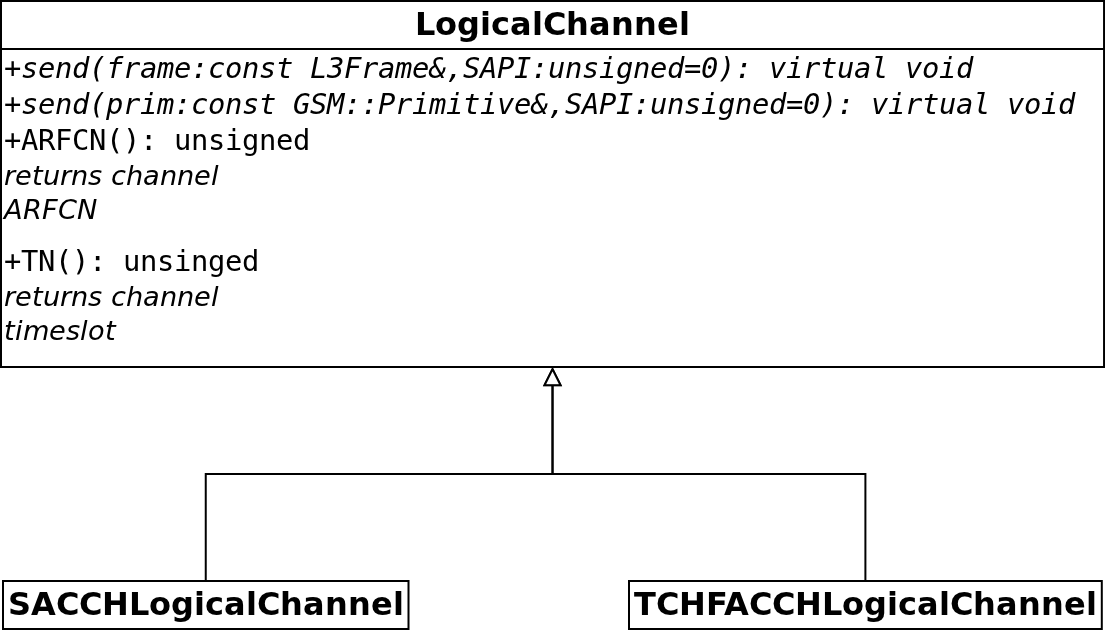
\includegraphics[width=0.9\textwidth]{img/lc}
  \caption{Klassendiagramm LogicalChannel}
  \label{fig:logchan}
\end{figure}

\subsection{L3Message-Klassen}

\begin{figure}[h!]
  \centering
  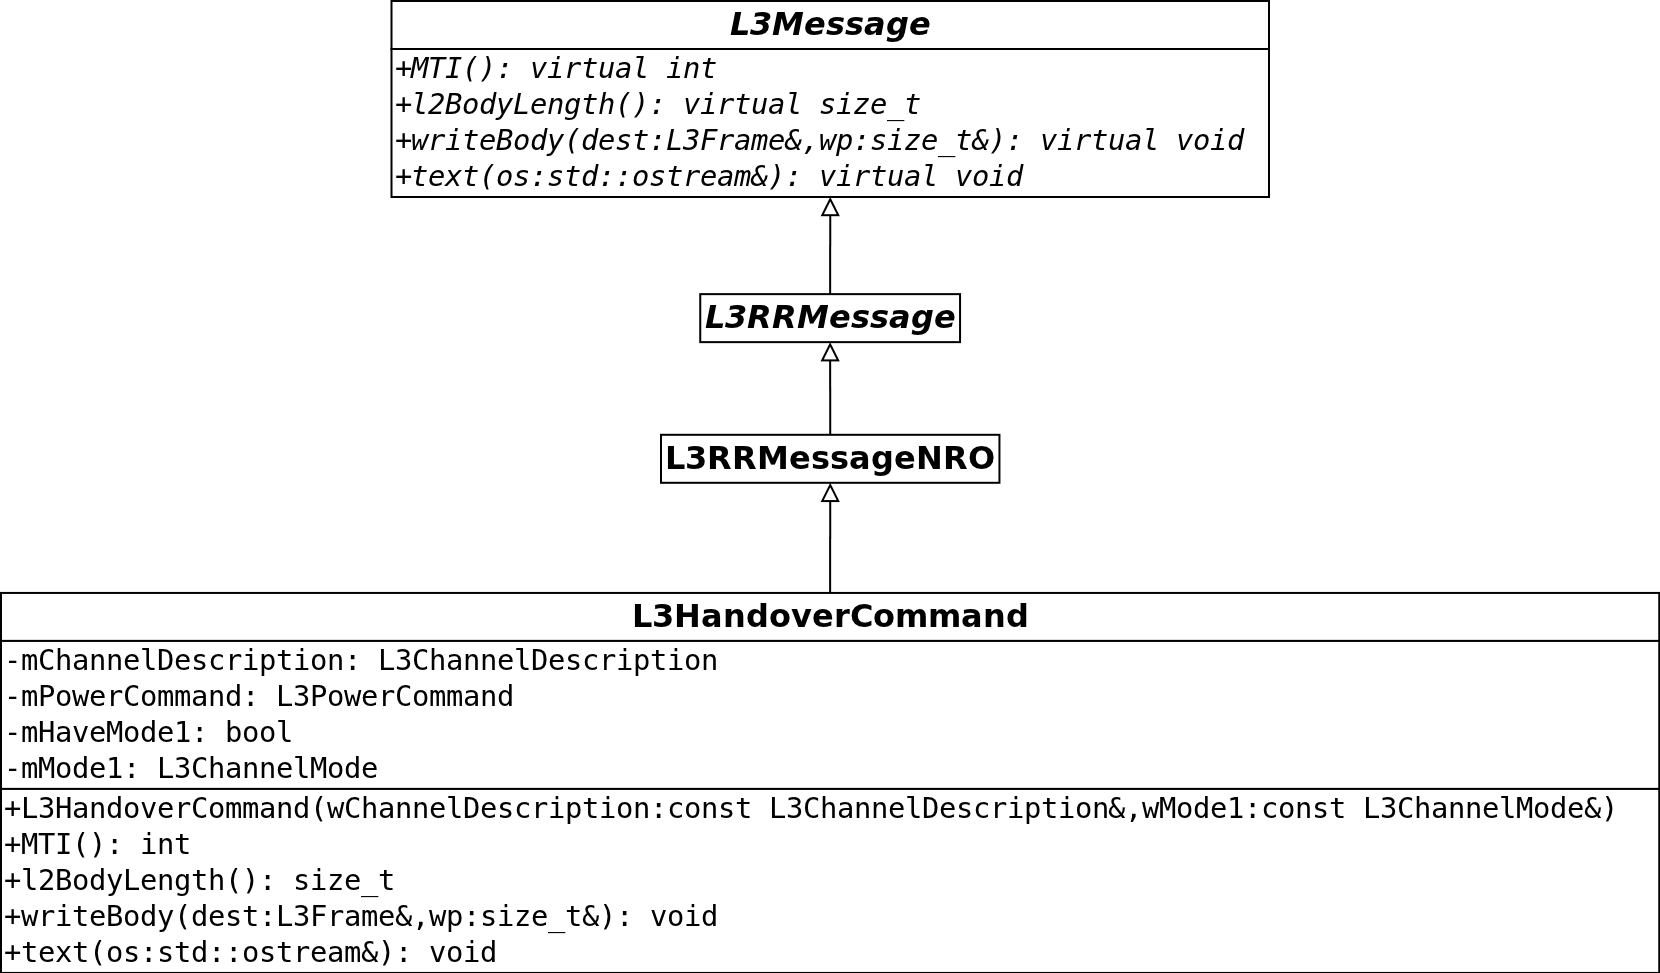
\includegraphics[width=0.9\textwidth]{img/l3m}
  \caption{Klassendiagramm L3Message}
  \label{fig:l3mess}
\end{figure}
